\section{Analisi dati su sitemi distribuiti}
\label{sec:analisi dati su sistemi distribuiti}
Il numero di utenti che ogni giorno spende bitcoin è in costante crescita. La tecnologia Bitcoin quindi è costretta a lavorare con volumi di dati sempre crescente. Per questo motivo, le applicazioni che fanno analisi devono adattarsi scegliendo sistemi consoni a queste moli di dati: i Sistemi distribuiti.
\\Esistono più definizioni (più o meno equivalenti fra loro) di un sistema distribuito, fra cui:
\begin{itemize}
\item  "Un sistema distribuito è una porzione di software che assicura che un insieme di calcolatori appaiano come un unico sistema coerente agli utenti del sistema stesso" (Maarten van Steen, 2016).\cite{sitema-distribuito-1}
\item "Un sistema distribuito consiste di un'insieme di calcolatori autonomi, connessi fra loro tramite una rete e un middleware di distribuzione, che permette ai computer di coordinare le loro attività e di condividere le risorse del sistema, in modo che gli utenti percepiscano il sistema come un unico servizio integrato di calcolo" (Wolfgang Emmerich, 1997).\cite{sitema-distribuito-2}
\item "Un sistema distribuito è un sistema in cui il fallimento di un computer che non sapevi neppure esistere può rendere il tuo computer inutilizzabile" (Leslie Lamport, 1987).\cite{sitema-distribuito-3}
\end{itemize}
Sintetizzando, un sistema distribuito è un insieme di processori indipendenti (con proprie risorse hardware/software) interconnessi da una rete di comunicazione, che cooperano per condividere alcune delle risorse ovunque distribuite ed eseguire algoritmi parallelamente. Questi sistemi riescono ad apparire all'utente come un singolo sistema, permettendo di avere una certa estrazione dall'harware dei singoli nodi.
\\I sistemi distribuiti [\ref{fig:sistemaDistr}] si contrappongo ai sistemi centralizzati, nella quale tutto il lavoro è eseguito da un solo calcolatore [\ref{fig:sistemaCentr}]. Un esempio di sistema distribuito è la rete Internet stessa, che si estende a livello mondiale comprendendo risorse fisicamente molto distanti tra loro, in cui processi con funzioni diverse e connessi da reti di vario tipo si scambiano messaggi informativi basati su disparati protocolli di comunicazione.
\begin{figure}[H]
     \subfloat[Sistema distribuito\label{fig:sistemaDistr}]{%
       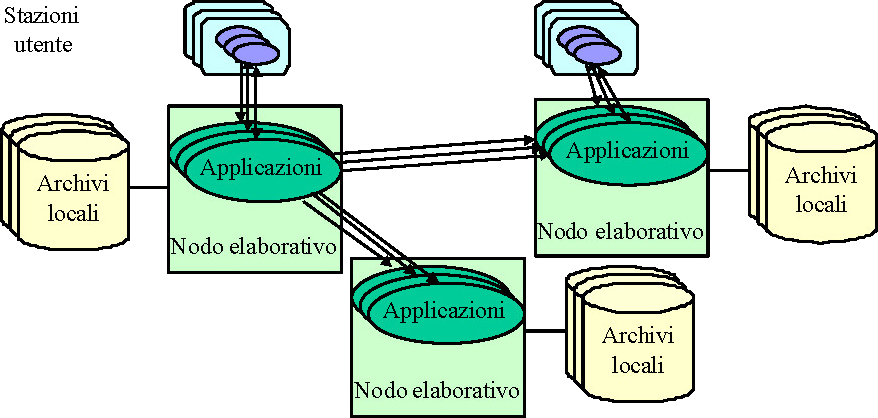
\includegraphics[width=0.50\textwidth]{images/sistemaDistr.png}
     }
     \hfill
     \subfloat[Sistema centralizzato\label{fig:sistemaCentr}]{%
       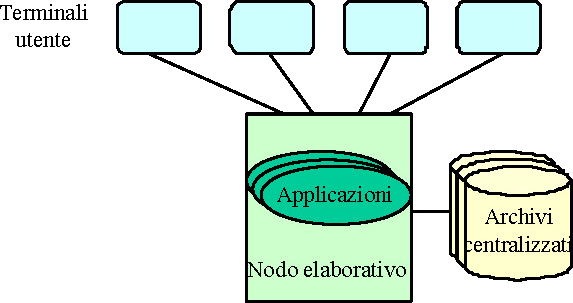
\includegraphics[width=0.50\textwidth]{images/sistemaCentr.png}
     }
     \caption{Differenza tra sistema distribuito e centralizzato.}
  	 \label{fig:sistemaDisCent}
\end{figure}
L'applicazione creata è eseguita su un sistema distribuito questo perché abbiamo bisogno di tempi di risposta bassi ed alta affidabilità dei dati. Per questo motivo il codice viene partizionato in piccoli problemi ed eseguiti dai nodi del nostro cluster. Il processo di partizione dei dati viene automatizzato dal framework Spark [\ref{sec:spark}] che si occupa della gestione, invio e recupero dei dati tra i vari nodi. 

\subsection{Caratteristiche di un sistema distribuito}
\label{subsec:caratteristiche di un sistema distribuito}
Un sistema distribuito si definisce tale se rispetta alcune caratteristiche come: 
\begin{itemize}
\item \textbf{Remoto}: le componenti di un sistema distribuito devono poter essere trattate allo stesso modo sia che siano in locale che in remoto.
\item \textbf{Concorrenza}: è possibile eseguire contemporaneamente due o più istruzioni su macchine differenti.
\item \textbf{Malfunzionamenti parziali}: Ogni componente del sistema può smettere di funzionare correttamente indipendentemente dalle altre componenti del sistema; questo non deve compromettere le funzionalità dell'intero sistema. I fallimenti che possono affliggere i processi possono essere di varia natura.
\item \textbf{Eterogeneità}: un sistema distribuito è eterogeneo per tecnologia sia hardware che software. Si realizza in tutti i contesti come rete di comunicazione, protocollo di rete, linguaggi di programmazione, applicazioni, etc.
\item \textbf{Autonomia}: un sistema distribuito non ha un singolo punto dal quale può essere controllato, coordinato e gestito. La collaborazione va ottenuta inviando messaggi tra le varie componenti del sistema e gestita tramite politiche di condivisione e di accesso che devono essere rigorosamente seguite. 
\item \textbf{Evoluzione}: un sistema distribuito può cambiare sostanzialmente durante la sua vita, sia perché cambia l'ambiente sia perché cambia la tecnologia utilizzata. L'obiettivo è quello di assecondare questi cambiamenti senza costi eccessivi.\cite{distSist:caratteristiche}
\end{itemize}

\subsection{Vantaggi e Svantaggi}
\label{subsec:vantaggi e svantaggi}
I sistemi distribuiti hanno dei pro e contro che sono da prendere in considerazione quando si vogliono adottare soluzioni di questo tipo.  
\\I vantaggi nell'utilizzo dei sistemi sono:
\begin{itemize}
\item \textbf{Connettività e collaborazione}: possibilità di condividere risorse hardware e software (compresi dati e applicazioni)
\item \textbf{Prestazioni e scalabilità}: la possibilità di aggiungere risorse, fornisce la capacità di migliorare le prestazioni e sostenere un carico che aumenta (scalabilità orizzontale)
\item \textbf{Tolleranza ai guasti}: grazie alla possibilità di replicare risorse e dati
\item \textbf{Apertura}: l'uso di protocolli standard aperti favorisce l'interoperabilità di hardware e software di fornitori diversi
\item \textbf{Economicità}: i sistemi distribuiti offrono spesso (ma non sempre) un miglior rapporto prezzo/qualità che i sistemi centralizzati basati su mainframe
\end{itemize}

Gli svantaggi invece sono:
\begin{itemize}
\item \textbf{Complessità}: i sistemi distribuiti sono più complessi di quelli centralizzati e quindi risultano più difficili da capire, inoltre, lo sviluppo delle applicazioni deve essere implementato ad hoc.
\item \textbf{Sicurezza}: l’accessibilità in rete pone problematiche di sicurezza
\item \textbf{Gestibilità}: è necessario uno sforzo maggiore per la gestione del sistema operativo e delle applicazioni
\end{itemize}
